\documentclass[a4paper,10pt]{scrartcl}

% Hier die Nummer des Blatts und Autoren angeben.
\newcommand{\blatt}{10}
\newcommand{\autor}{Jim Martens}

\usepackage{hci}
\usepackage[utf8]{inputenc}
\usepackage{float}
\usepackage[official]{eurosym}
\usepackage[parfill]{parskip}

\begin{document}
% Seitenkopf mit Informationen
\kopf
\renewcommand{\figurename}{Figure}

\aufgabe{1}

\subsection*{Website}

Bei der Website habe ich mich für die 404-Errorseite von gog.com entschieden, da bei dieser nicht all zu viel vorhanden ist und damit eine Analyse halbwegs gerechtfertigt erscheint.

Oben in der Menüleiste kann man das Logo sehen, welches bei Klick darauf wieder zur Startseite führt. Dies entspricht damit mehreren Pattern (Escape Hatch, Pyramid). Außerdem ist die gesamte Menüleiste ein ActionPanel, da es stets am oberen Rand verbleibt und damit immer zu sehen ist.

Der Hauptbereich der Seite entspricht einer CenterStage, da alles Wesentliche in der horizontalen und vertikalen Mitte angeordnet ist. Die Suche in der oberen Leiste implementiert AutoCompletion (hier nicht zu sehen).
\begin{figure}[htp]
	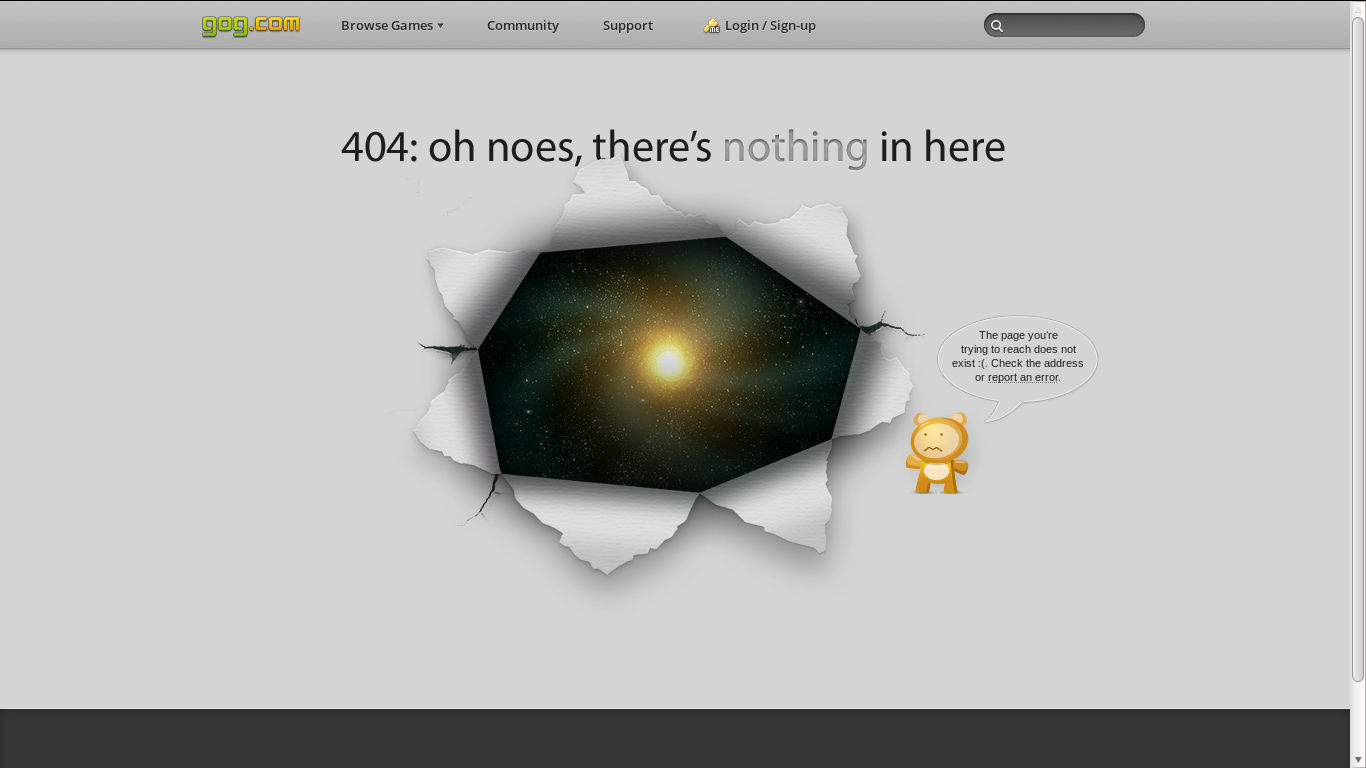
\includegraphics[scale=0.35]{ID-GOG-404}
\end{figure}

\subsection*{Desktop-Anwendung}

Bei der Desktopanwendung habe ich mich für Gimp entschieden.

Leicht zu erkennen sind die Pattern Canvas Plus Palette und Movable Panels. Ebenso lassen sich Module Tabs in dem Panel auf der rechten Seite erkennen.
In jenem Panel können auch zwei ButtonGroups erkannt werden.

Am unteren Rand kann eine SpinBox, sowie eine N-Item Drop-Down-List gesehen werden.
 
\begin{figure}[htp]
	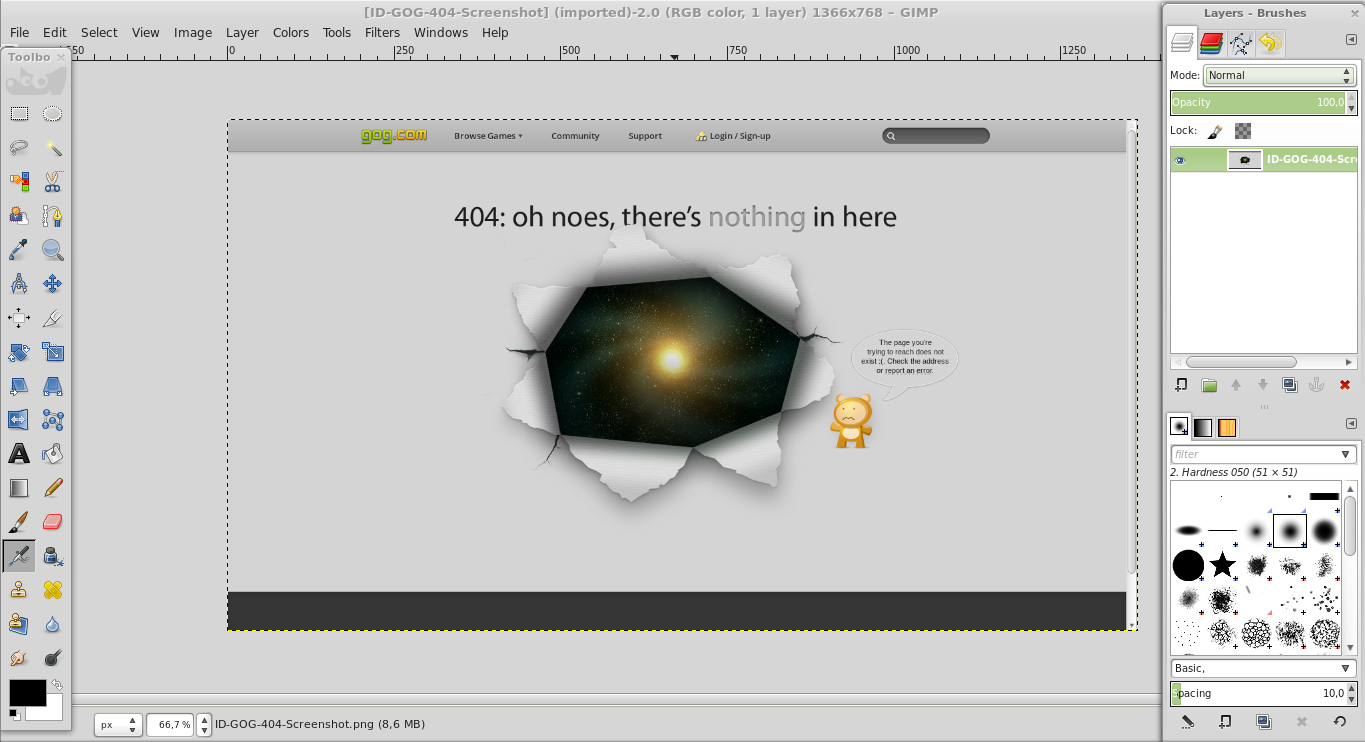
\includegraphics[scale=0.35]{ID-Gimp}
\end{figure}

\newpage
\subsection*{Mobile Anwendung}

Bei dieser Anwendung kann am oberen Rand eine ButtonGroup sehen. Außerdem wird die Sequence Map verwendet, indem man zurück zur Reiseauskunft navigieren kann. Zudem gibt es eine ButtonGroup in der unteren Leiste.

\begin{figure}[htp]
	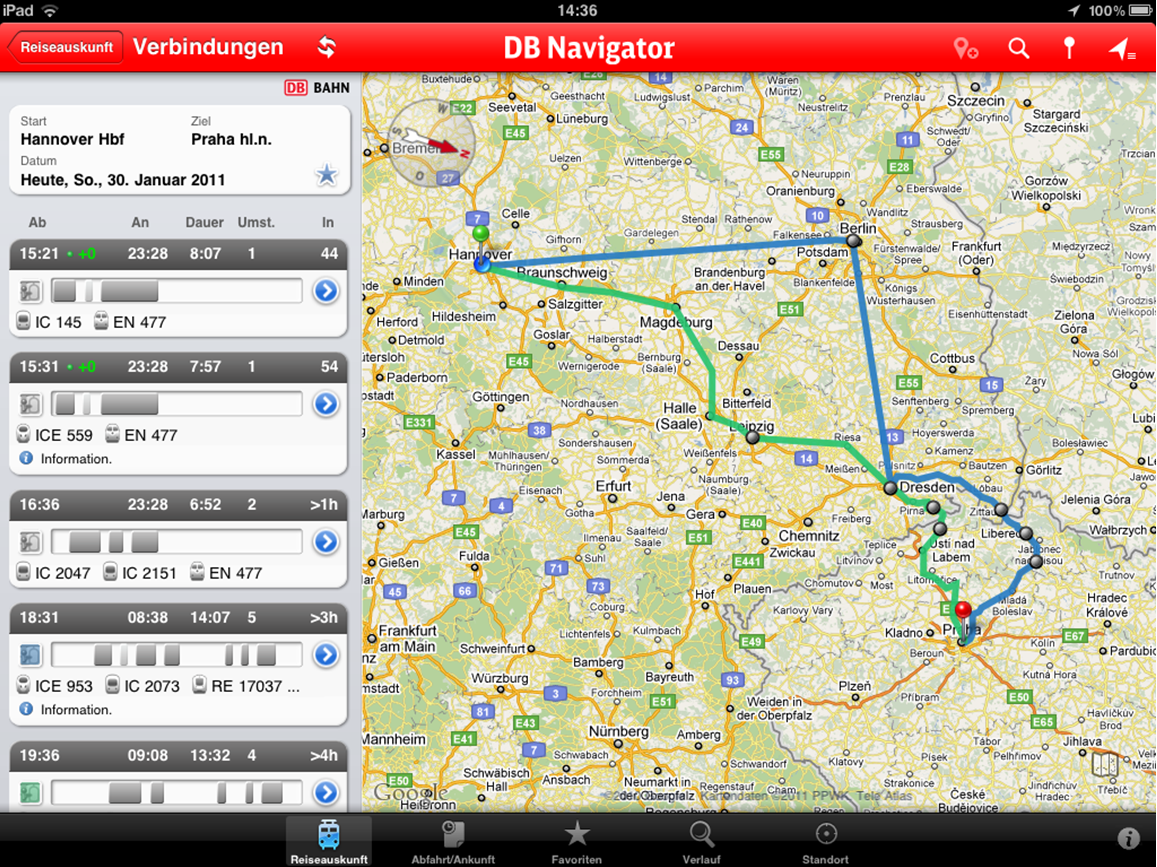
\includegraphics[scale=0.40]{ID-DBNavigator}
	\caption{Quelle: http://www.hacon.de/hafas-en/mobil/HaCon\%20iPad\%20Mockup\%201.png}
\end{figure}

\end{document}